% Allow relative paths in included subfiles that are compiled separately
% See https://tex.stackexchange.com/questions/153312/
\providecommand{\main}{..}
\documentclass[\main/thesis.tex]{subfiles}

\begin{document}

\chapter{Autoencoder Embeddings with Improved Tree Ensemble}
\chaptermark{AENCXGB}
\label{chp:aencxgb}

In Chapter~\ref{chp:dl_autoenc} I discovered that the autoencoder classification models provided worse overall challenge metrics compared to the gradient boosted tree model proposed in Chapter~\ref{chp:xgbensemble}, but are more sensitive in detecting \gls{irbbb}, \gls{lanfb}, and \gls{rad}.

This chapter explores the effectiveness of combining the autoencoder learned embeddings with the manually engineered features to train a new set of gradient boosted tree models.
I extend the approaches used in Chapters~\ref{chp:xgbensemble} and \ref{chp:dl_autoenc} with the following research predictions:
\begin{enumerate}[label=RQ\arabic*,itemindent=0.8em,start=1]
    \item \label{question:xgb_aenc_avg_vs_lab} What is the effect of selecting top features with respect to the label-wise classifiers, compared to averaging the feature importances over all classifiers?
    I predict that labelwise selection of important features will result in an improved classifier, providing a statistically significant higher challenge metric with a mean difference of over 0.01.
    \item \label{question:xgb_aenc_pruning} How important is feature selection when evaluating the classifier challenge metric?
    I predict that classifiers that do not perform any feature selection will have a statistically significant lower challenge metric than classifiers that perform feature selection, but there will be no significant difference between aggressive pruning (top 100 features) and moderate pruning (top 1000 features).
    \item \label{question:xgb_aenc_embd_vs_no_embd} Will incorporating the sequence embeddings from our deep learning autoencoder improve classification challenge metric?
    Aligning with my thesis statement, I predict that adding in the deep learning autoencoder will statistically significantly increase the overall challenge metric of the classifiers.
    % \item \label{question:xgb_aenc_embd_ratio} When adding the deep learning generated autoencoder embeddings, are they represented proportionally relative to the standard 12-lead derived heart beat, heart rate, and full waveform derived feature categories?
\end{enumerate}

\section{Methodology}
\label{sec:aencxgb_methodology}

I combine the techniques applied in Section~\ref{ssec:xgb_feature_engineering} and Section~\ref{ssec:aenc_seq_embedding} to convert the variable length features into fixed length input vectors for all \gls{ecg} records.

This chapter focuses on the training of \texttt{xgboost}~\cite{chen_xgboost_2016} binary classifiers for each of the 27 labels selected by the PhysioNet/CinC challenge.
I explore ten different configurations of the tabular inputs:
\begin{enumerate}
    \item \label{item:xgb_aenc_model_all_w_embd} \textbf{All Features with Embeddings}: I combine the heartbeat features, heart rate variability features, and overall waveform features input vector used in Section~\ref{ssec:xgb_feature_engineering} (size 18,950) with the autoencoder sequence embedding vector (size 768) to create a combined input vector of size 19,718 and train an XGBoost classifier for each of the 27 diagnosed labels.
    These label-wise classifiers provide feature importances for use in configurations~\ref{item:xgb_aenc_model_avgd_top_1000_w_embd},~\ref{item:xgb_aenc_model_top_1000_w_embd},~\ref{item:xgb_aenc_model_avgd_top_100_w_embd},~and~\ref{item:xgb_aenc_model_top_100_w_embd}.
    \item \label{item:xgb_aenc_model_all_no_embd} \textbf{All Features}: I only use the heartbeat features, heart rate variability features, and overall waveform features to create an input vector of size 18,950 as the input to our label-wise XGBoost classifier ensembles. One XGBoost classifier is trained per label. This configuration is identical to the Phase 1 methodology described in Section~\ref{ssec:xgb_classification}.
    The trained classifiers are subsequently used to provide feature importances for configurations~\ref{item:xgb_aenc_model_avgd_top_1000_no_embd},~\ref{item:xgb_aenc_model_top_1000_no_embd},~\ref{item:xgb_aenc_model_avgd_top_100_no_embd},~and~\ref{item:xgb_aenc_model_top_100_no_embd}.
    \item \label{item:xgb_aenc_model_avgd_top_1000_w_embd} \textbf{Averaged Top 1000 Features with Embeddings}: Using the trained models from Configuration~\ref{item:xgb_aenc_model_all_w_embd}, all label-wise classifier feature importances provided by the XGBoost classifiers are averaged together before selecting the top 1,000 features. Using this averaged overall set of 1,000 most important features, one XGBoost classifier is trained per label.
    \item \label{item:xgb_aenc_model_top_1000_w_embd} \textbf{Top 1000 Features with Embeddings}: Starting from Configuration~\ref{item:xgb_aenc_model_all_w_embd}, I select the top 1,000 features for each XGBoost diagnosis classifier and retrain a new set of 27 classifiers using the reduced feature set. One XGBoost classifier is trained per label only using the importances of the parent model sharing the same label.
    \item \label{item:xgb_aenc_model_avgd_top_100_w_embd} \textbf{Averaged Top 100 Features with Embeddings}: Using the trained models from Configuration~\ref{item:xgb_aenc_model_all_w_embd}, all label-wise XGBoost classifier feature importances are averaged together before selecting the top 100 features. One XGBoost classifier is trained per label using the averaged 100 most important features of all parent XGBoost label-to-classifier pairs.
    \item \label{item:xgb_aenc_model_top_100_w_embd} \textbf{Top 100 Features with Embeddings}: Starting from Configuration~\ref{item:xgb_aenc_model_all_w_embd}, I select the 100 most important features for each XGBoost diagnosis classifier and retrain a new set of 27 classifiers.
    A separate XGBoost classifier is trained per label using the 100 most important features of the parent classifier sharing the same label.
    \item \label{item:xgb_aenc_model_avgd_top_1000_no_embd} \textbf{Averaged Top 1000 Features}: Using Configuration~\ref{item:xgb_aenc_model_all_no_embd}, the XGBoost classifier feature importances for all labels are averaged together to select the top 1,000 features. These 1,000 features are used to train a new model for each label. This configuration is identical to the Phase 2 methodology described in Section~\ref{ssec:xgb_classification}.
    \item \label{item:xgb_aenc_model_top_1000_no_embd} \textbf{Top 1000 Features}: Starting from Configuration~\ref{item:xgb_aenc_model_all_no_embd}, a new set of 27 XGBoost classifiers are trained using the reduced top 1,000 most important features per label classifier.
    One model is trained per label using only the top 1,000 features of the parent model sharing the same label.
    \item \label{item:xgb_aenc_model_avgd_top_100_no_embd} \textbf{Averaged Top 100 Features}: Using Configuration~\ref{item:xgb_aenc_model_all_no_embd}, the XGBoost classifier feature importances for all labels are averaged together to select the top 100 features.
    Using the averaged 100 most important features of all classifiers, a model is trained for each label.
    \item \label{item:xgb_aenc_model_top_100_no_embd} \textbf{Top 100 Features}: Starting from Configuration~\ref{item:xgb_aenc_model_all_no_embd}, a new set of 27 classifiers are trained using the reduced top 100 most important features per XGBoost binary label classifier.
    The reduced set of 100 features are specific to the label and are not averaged together between other classifiers.
\end{enumerate}

The significant differences distinguishing these approaches from the top 1000 features approach used in Section~\ref{ssec:xgb_classification} are that the importances of features for each of the labels are now evaluated independently, where the prior experiment used the same reduced set of features for all classifiers.

The ``gain'' feature importance is used.
This is the relative contribution of the provided feature to the overall model, defined as the sum of each feature's contribution for every tree in the XGBoost classifier.

I further revise the inadequate dataset partitioning to use Monte Carlo cross-validation 20 times, randomly partitioning the available corpus of public data into 80\% training, 10\% validation, and 10\% test splits.

For each experiment configuration run, I train an XGBoost binary classifier for each of the 27 diagnosed labels.
I use the dropout augmented regression tree booster proposed by Vinayak and Gilad-Bachrach~\cite{vinayak_dart_2015} and sample the training instances using probabilities proportional to the training gradients.
I use the scoring function reward matrix weights from Figure~\ref{fig:reward_matrix} as instance sample weights, capping positive examples to a threshold of 0.5.
I further scale the positive samples using the ratio of negative samples over positive samples for the given label and dataset split.
During training, if the evaluation set binary logistic regression loss fails to improve after 20 epochs of training, we early stop to mitigate overfitting on the training set.

\section{Results}
\label{sec:xgb_aenc_results}

\begin{figure}[h]
    \centering
    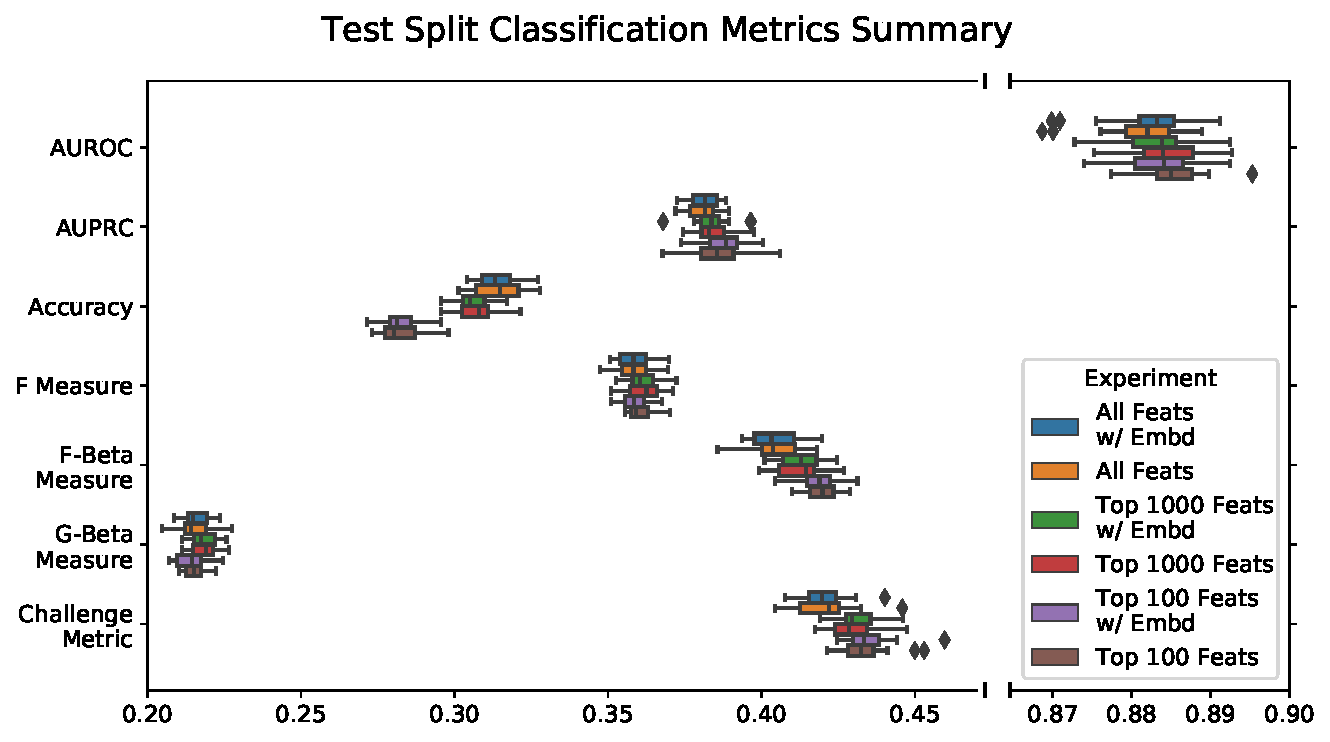
\includegraphics[trim={0.2cm 0.3cm 0.2cm 0.1cm},clip,width=\textwidth]{figure/xgb_aenc_classification_metrics.pdf}
    \caption[Test split classification metrics of XGB ensemble using all configurations of engineered features and autoencoder embeddings.]{Test split classification metrics of XGB ensemble using
    Configuration~\ref{item:xgb_aenc_model_all_w_embd}: All Features with Embeddings;
    Configuration~\ref{item:xgb_aenc_model_all_no_embd}: All Features;
    Configuration~\ref{item:xgb_aenc_model_avgd_top_1000_w_embd}: Averaged Top 1000 Features with Embeddings;
    Configuration~\ref{item:xgb_aenc_model_top_1000_w_embd}: Top 1000 Features with Embeddings;
    Configuration~\ref{item:xgb_aenc_model_avgd_top_100_w_embd}: Averaged Top 100 Features with Embeddings;
    Configuration~\ref{item:xgb_aenc_model_top_100_w_embd}: Top 100 Features with Embeddings;
    Configuration~\ref{item:xgb_aenc_model_avgd_top_1000_no_embd}: Averaged Top 1000 Features;
    Configuration~\ref{item:xgb_aenc_model_top_1000_no_embd}: Top 1000 Features;
    Configuration~\ref{item:xgb_aenc_model_avgd_top_100_no_embd}: Averaged Top 100 Features; and
    Configuration~\ref{item:xgb_aenc_model_top_100_no_embd}: Top 100 Features.
    }
    \label{fig:xgb_aenc_classification_metrics}
\end{figure}

\begin{table}[t]
    \caption{\label{tab:xgb_aenc_classification_metrics} Test split classification metrics mean ($\bar{x}$) and standard deviations ($\sigma$) for all experiment configurations. Bolded value indicates largest mean for metric category.}
    \vspace{2 mm}
    \centerline{\begin{tabular}{@{}c@{{ }}r@{{ }}c|c@{{ }}c@{{ }}c@{{ }}c@{{ }}c@{{ }}c@{{ }}c@{}}
    \multirow{2}{*}{\textbf{\#}}& \multirow{2}{*}{\textbf{Experiment}} & & \multirow{2}{*}{\textbf{AUROC}} & \multirow{2}{*}{\textbf{AUPRC}} & \multirow{2}{*}{\textbf{Accuracy}} & \multirow{2}{*}{\textbf{F Measure}} & \multirow{2}{*}{\textbf{F-Beta}} & \multirow{2}{*}{\textbf{G-Beta}} & \textbf{Challenge} \\
    & & & & & & & & & \textbf{Metric} \\ \hline
    % Configuration 1
    \multirow{2}{*}{\ref{item:xgb_aenc_model_all_w_embd}} & All Feats & $\bar{x}$ & $0.8821$ & $0.3813$ & $0.3137$ & $0.3587$ & $0.4047$ & $0.2160$ & $0.4207$ \\
    & w/ Embd & $\sigma$ & $5.3 \mathrm{E}{-3}$ & $4.9 \mathrm{E}{-3}$ & $6.8 \mathrm{E}{-3}$ & $5.9 \mathrm{E}{-3}$ & $8.1 \mathrm{E}{-3}$ & $3.9 \mathrm{E}{-3}$ & $7.7 \mathrm{E}{-3}$
    \\ \hline
    % Configuration 2
    \multirow{2}{*}{\ref{item:xgb_aenc_model_all_no_embd}} & \multirow{2}{*}{All Feats} & $\bar{x}$ & $0.8815$ & $0.3809$ & \textbf{0.3139} & $0.3582$ & $0.4036$ & $0.2150$ & $0.4206$ \\
    & & $\sigma$ & $5.5 \mathrm{E}{-3}$ & $5.0 \mathrm{E}{-3}$ & $7.9 \mathrm{E}{-3}$ & $6.0 \mathrm{E}{-3}$ & $8.6 \mathrm{E}{-3}$ & $5.2 \mathrm{E}{-3}$ & $1.0 \mathrm{E}{-2}$ \\ \hline
    % Configuration 3
    \multirow{2}{*}{\ref{item:xgb_aenc_model_avgd_top_1000_w_embd}} & Avg Top 1000 & $\bar{x}$ & \textbf{0.8876} & \textbf{0.3900} & $0.3068$ & $0.3637$ & $0.4165$ & \textbf{0.2194} & \textbf{0.4366} \\
    & Feats w/ Embd & $\sigma$ & $4.6 \mathrm{E}{-3}$ & $5.5 \mathrm{E}{-3}$ & $6.5 \mathrm{E}{-3}$ & $4.5 \mathrm{E}{-3}$ & $6.0 \mathrm{E}{-3}$ & $4.3 \mathrm{E}{-3}$ & $7.1 \mathrm{E}{-3}$ \\ \hline
    % Configuration 4
    \multirow{2}{*}{\ref{item:xgb_aenc_model_top_1000_w_embd}} & Top 1000 Feats & $\bar{x}$ & $0.8836$ & $0.3837$ & $0.3062$ & $0.3613$ & $0.4128$ & $0.2183$ & $0.4316$ \\
    & w/ Embd & $\sigma$ & $4.8 \mathrm{E}{-3}$ & $6.4 \mathrm{E}{-3}$ & $5.4 \mathrm{E}{-3}$ & $5.4 \mathrm{E}{-3}$ & $6.7 \mathrm{E}{-3}$ & $4.3 \mathrm{E}{-3}$ & $7.0 \mathrm{E}{-3}$ \\ \hline
    % Configuration 5
    \multirow{2}{*}{\ref{item:xgb_aenc_model_avgd_top_100_w_embd}} & Avg Top 100 & $\bar{x}$ & $0.8740$ & $0.3740$ & $0.2800$ & $0.3482$ & $0.4062$ & $0.2066$ & $0.4215$ \\
    & Feats w/ Embd & $\sigma$ & $5.1 \mathrm{E}{-3}$ & $7.8 \mathrm{E}{-3}$ & $9.7 \mathrm{E}{-3}$ & $6.5 \mathrm{E}{-3}$ & $6.8 \mathrm{E}{-3}$ & $5.2 \mathrm{E}{-3}$ & $9.9 \mathrm{E}{-3}$ \\ \hline
    % Configuration 6
    \multirow{2}{*}{\ref{item:xgb_aenc_model_top_100_w_embd}} & Top 100 Feats & $\bar{x}$ & $0.8836$ & $0.3876$ & $0.2820$ & $0.3588$ & $0.4190$ & $0.2143$ & $0.4348$ \\
    & w/ Embd & $\sigma$ & $4.9 \mathrm{E}{-3}$ & $7.0 \mathrm{E}{-3}$ & $6.2 \mathrm{E}{-3}$ & $5.1 \mathrm{E}{-3}$ & $6.8 \mathrm{E}{-3}$ & $4.9 \mathrm{E}{-3}$ & $7.8 \mathrm{E}{-3}$ \\ \hline
    % Configuration 7
    \multirow{2}{*}{\ref{item:xgb_aenc_model_avgd_top_1000_no_embd}} & Avg Top & $\bar{x}$ & $0.8871$ & $0.3890$ & $0.3085$ & \textbf{0.3640} & $0.4165$ & $0.2187$ & $0.4358$ \\
    & 1000 Feats & $\sigma$ & $5.1 \mathrm{E}{-3}$ & $6.7 \mathrm{E}{-3}$ & $6.6 \mathrm{E}{-3}$ & $6.2 \mathrm{E}{-3}$ & $8.1 \mathrm{E}{-3}$ & $5.6 \mathrm{E}{-3}$ & $8.1 \mathrm{E}{-3}$ \\ \hline
    % Configuration 8
    \multirow{2}{*}{\ref{item:xgb_aenc_model_top_1000_no_embd}} & \multirow{2}{*}{Top 1000 Feats} & $\bar{x}$ & $0.8843$ & $0.3836$ & $0.3075$ & $0.3619$ & $0.4126$ & $0.2179$ & $0.4295$ \\
    & & $\sigma$ & $5.2 \mathrm{E}{-3}$ & $5.6 \mathrm{E}{-3}$ & $6.4 \mathrm{E}{-3}$ & $5.2 \mathrm{E}{-3}$ & $7.5 \mathrm{E}{-3}$ & $4.4 \mathrm{E}{-3}$ & $8.1 \mathrm{E}{-3}$ \\ \hline
    % Configuration 9
    \multirow{2}{*}{\ref{item:xgb_aenc_model_avgd_top_100_no_embd}} & Avg Top & $\bar{x}$ & $0.8714$ & $0.3748$ & $0.2800$ & $0.3471$ & $0.4035$ & $0.2057$ & $0.4195$ \\
    & 100 Feats & $\sigma$ & $6.7 \mathrm{E}{-3}$ & $6.4 \mathrm{E}{-3}$ & $5.3 \mathrm{E}{-3}$ & $4.6 \mathrm{E}{-3}$ & $6.2 \mathrm{E}{-3}$ & $5.1 \mathrm{E}{-3}$ & $7.8 \mathrm{E}{-3}$ \\ \hline
    % Configuration 10
    \multirow{2}{*}{\ref{item:xgb_aenc_model_top_100_no_embd}} & \multirow{2}{*}{Top 100 Feats} & $\bar{x}$ & $0.8848$ & $0.3857$ & $0.2830$ & $0.3604$ & \textbf{0.4198} & $0.2150$ & $0.4335$ \\
    & & $\sigma$ & $4.5 \mathrm{E}{-3}$ & $8.5 \mathrm{E}{-3}$ & $7.5 \mathrm{E}{-3}$ & $4.0 \mathrm{E}{-3}$ & $5.3 \mathrm{E}{-3}$ & $3.3 \mathrm{E}{-3}$ & $8.2 \mathrm{E}{-3}$ \\
    \end{tabular}}
\end{table}

\begin{figure}[t]
    \centering
    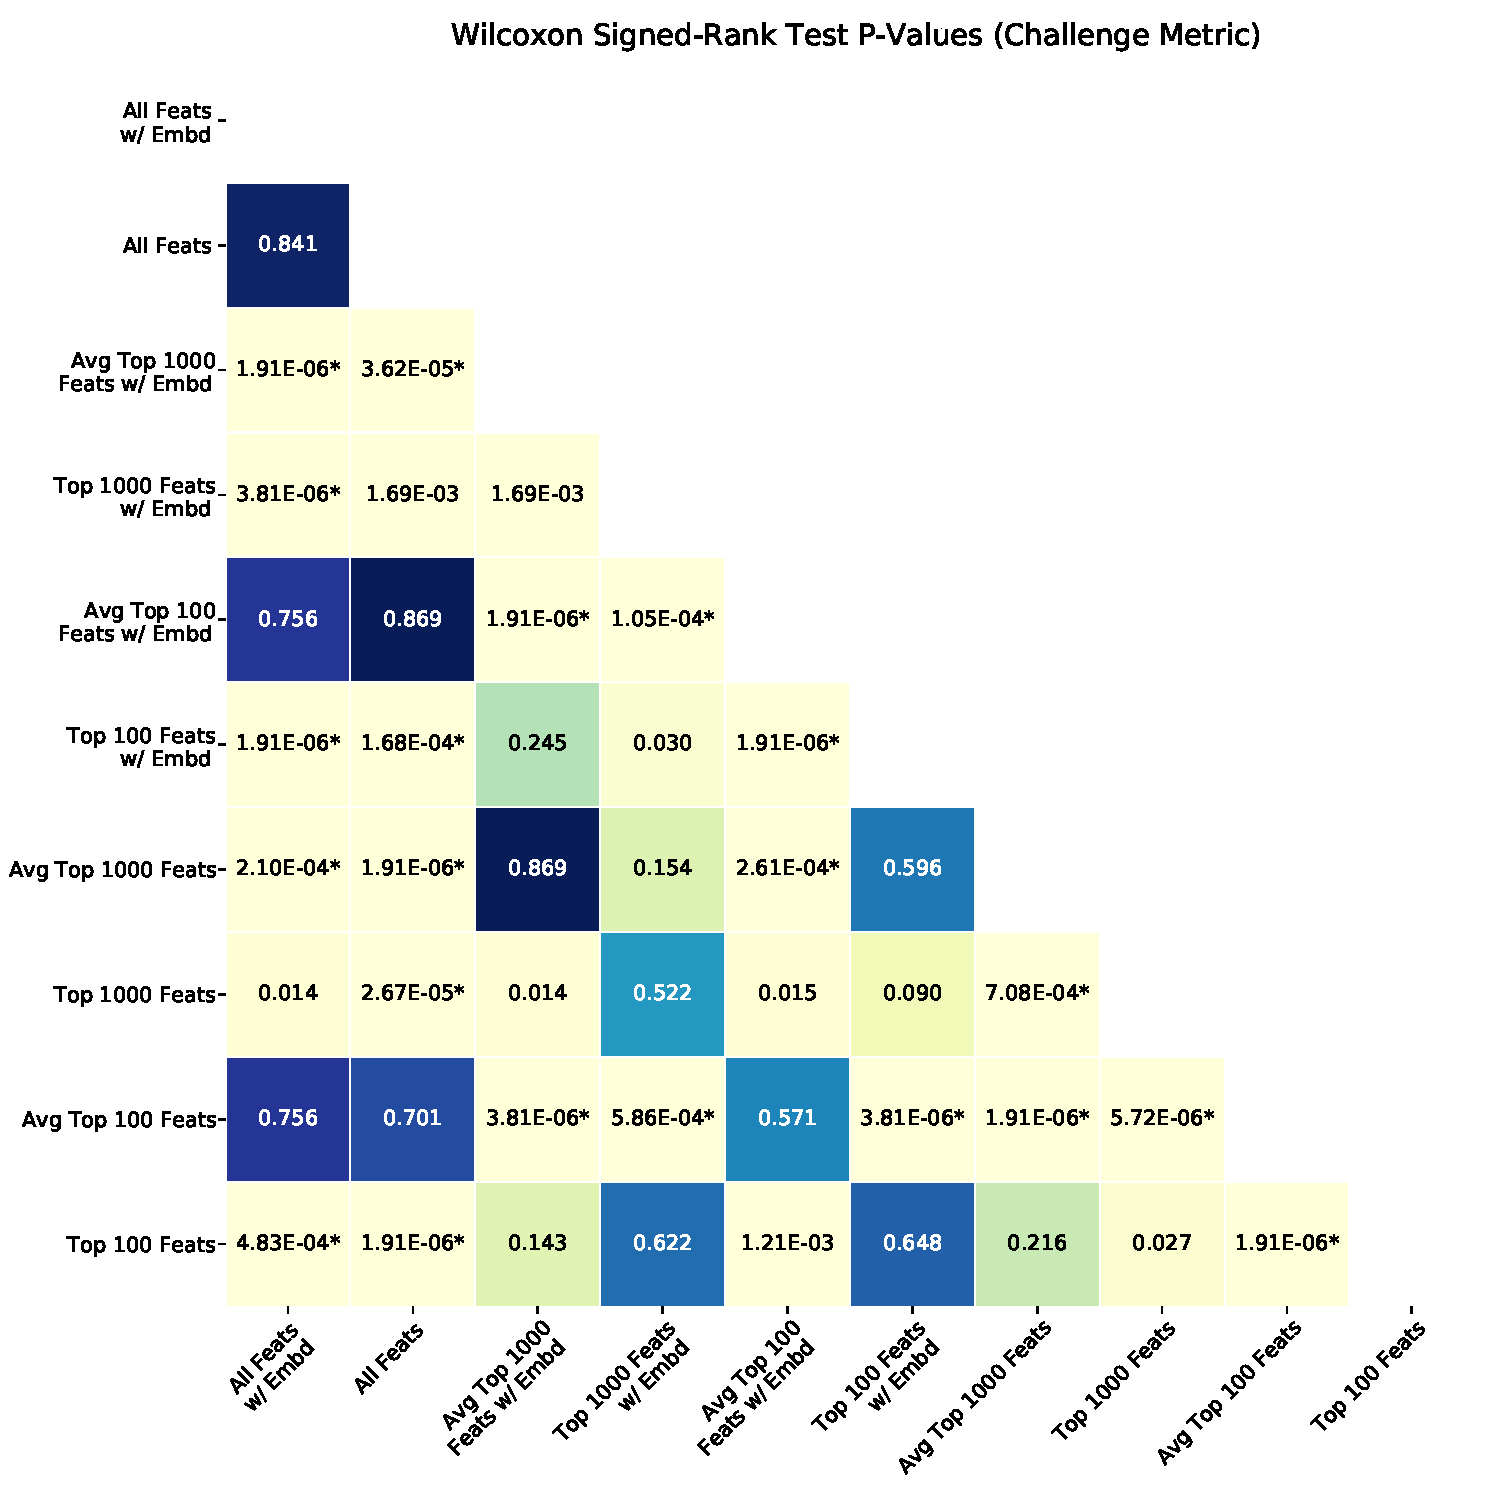
\includegraphics[width=12cm]{figure/xgb_aenc_wilcoxon_srt_p_vals.pdf}
    \caption[Wilcoxon signed-rank test P-values, comparing test split challenge metric distributions of all 6 experiment configurations.]{Wilcoxon signed-rank test P-values, comparing test split challenge metric distributions of all 6 experiment configurations. Asterisk indicates significantly different challenge metric distribution at an alpha of 0.001.}
    \label{fig:xgb_aenc_wilcoxon_srt_p_vals}
\end{figure}

Refer to Figure~\ref{fig:xgb_aenc_classification_metrics} and Table~\ref{tab:xgb_aenc_classification_metrics} for the test set split classification metric summaries for all experiment configurations.
The experiment configuration with the largest mean challenge score is Configuration~\ref{item:xgb_aenc_model_avgd_top_1000_w_embd} ``Averaged Top 1000 Features with Embeddings", or the top 1000 features from both the engineered and autoencoder sources.
Although Configuration~\ref{item:xgb_aenc_model_avgd_top_1000_w_embd} has the highest mean challenge score, it is only statistically different compared to Configurations~\ref{item:xgb_aenc_model_all_w_embd}, \ref{item:xgb_aenc_model_all_no_embd}, \ref{item:xgb_aenc_model_avgd_top_100_w_embd}, and \ref{item:xgb_aenc_model_top_100_no_embd}.
See Figure~\ref{fig:xgb_aenc_wilcoxon_srt_p_vals} for the Wilcoxon signed-rank test evaluated on all configuration pairs.

\subsection{Averaged vs Labelwise Feature Selection}
For \ref{question:xgb_aenc_avg_vs_lab}, I investigate if selecting important features by classifier is an improvement to just averaging all of the classifiers together.
If my prediction holds true, I expect to see the averaged top feature configurations perform worse than the top feature configurations.
With an alpha of $0.001$, I analyze the relevant configuration pairs:
\begin{itemize}
    \item \textbf{1000 Features with Embeddings}: Configuration~\ref{item:xgb_aenc_model_avgd_top_1000_w_embd} has a higher challenge score than Configuration~\ref{item:xgb_aenc_model_top_1000_w_embd}, but it is not statistically significant.
    \item \textbf{100 Features with Embeddings}: Configuration~\ref{item:xgb_aenc_model_avgd_top_100_w_embd} has a lower challenge score than Configuration~\ref{item:xgb_aenc_model_top_100_w_embd}, and \emph{it is statistically significant}, suggesting labelwise selection of features increases the challenge metric.
    \item \textbf{1000 Features}: Configuration~\ref{item:xgb_aenc_model_avgd_top_1000_no_embd} has a higher challenge score than Configuration~\ref{item:xgb_aenc_model_top_1000_no_embd}, and \emph{it is statistically significant}, suggesting labelwise selection of features decreases the challenge metric.
    \item \textbf{100 Features}: Configuration~\ref{item:xgb_aenc_model_avgd_top_100_no_embd} has a lower challenge score than Configuration~\ref{item:xgb_aenc_model_top_100_no_embd}, and \emph{it is statistically significant}, suggesting labelwise selection of features increases the challenge metric.
\end{itemize}

\ref{question:xgb_aenc_avg_vs_lab}: When the feature pruning is not aggressive, such as taking the top 1000 features, the improvement in the challenge metric score is inconsistent resulting in no clear conclusion.
Labelwise selection of features results in a significantly higher challenge metric for the ``100 Features with Embeddings'' and ``100 Features'' configurations, suggesting that labelwise selection of features improves classifier performance when the feature pruning is aggressive.

\subsection{Effectiveness of Feature Selection}
In \ref{question:xgb_aenc_pruning}, I hypothesize that reducing the number of features passed to the classifier from the original unpruned set of features will improve the challenge metric.
If my prediction is accurate, I expect to see the models using ``All Features'' and ``All Features with Embeddings'' to have lower challenge scores than all other configurations.
Using an alpha of $0.001$, I compare the appropriate configurations:
\begin{itemize}
    \item \textbf{From All to Top 1000}: Configuration~\ref{item:xgb_aenc_model_all_w_embd} has a \emph{statistically significant} lower challenge score than Configurations~\ref{item:xgb_aenc_model_avgd_top_1000_w_embd}~and~\ref{item:xgb_aenc_model_top_1000_w_embd}, suggesting that pruning from all 19,718 features down to the top 1000 features is effective in improving the classifier's challenge score.
    In addition, the non-embedding variants Configuration~\ref{item:xgb_aenc_model_all_no_embd} also has a \emph{statistically significant} lower challenge score compared to Configurations~\ref{item:xgb_aenc_model_avgd_top_1000_no_embd}~and~\ref{item:xgb_aenc_model_top_1000_no_embd}, suggesting that a moderate pruning from all 18,950 features down to the top 1000 features is effective in improving the classifier's challenge score.
    \item \textbf{From All to Top 100}: Configuration~\ref{item:xgb_aenc_model_all_w_embd} has a lower challenge score than Configurations~\ref{item:xgb_aenc_model_avgd_top_100_w_embd}~and~\ref{item:xgb_aenc_model_top_100_w_embd}, however it is only statistically significant when compared with Configuration~\ref{item:xgb_aenc_model_top_100_w_embd} that performs labelwise selection of feature importances.
    When looking at the non-embedding variants, Configuration~\ref{item:xgb_aenc_model_all_no_embd} has a \emph{statistically significant} lower challenge score than Configuration~\ref{item:xgb_aenc_model_top_100_no_embd}, but no significant difference when compared to Configuration~\ref{item:xgb_aenc_model_avgd_top_100_no_embd}.
    These comparisons suggest that when performing aggressive pruning down to a subset of 100 features, the classifier's challenge metric score improves only if labelwise feature selection is applied.
    \item \textbf{From Top 1000 to Top 100}: Configuration~\ref{item:xgb_aenc_model_avgd_top_1000_w_embd} has a \emph{statistically significant} higher challenge score compared to Configuration~\ref{item:xgb_aenc_model_avgd_top_100_w_embd}.
    Configuration~\ref{item:xgb_aenc_model_top_1000_w_embd} has no significant difference in challenge score compared to Configuration~\ref{item:xgb_aenc_model_top_100_w_embd}.
    Configuration~\ref{item:xgb_aenc_model_avgd_top_1000_no_embd} has a \emph{statistically significant} higher challenge score compared to Configuration~\ref{item:xgb_aenc_model_avgd_top_100_no_embd}.
    No significant difference in challenge score is found between Configuration~\ref{item:xgb_aenc_model_top_1000_no_embd} and Configuration~\ref{item:xgb_aenc_model_top_100_no_embd}.
\end{itemize}

\ref{question:xgb_aenc_pruning}: When pruning from all available features, moderate pruning to reduce the feature space to 1000 inputs is effective in improving the challenge score of the classifiers.
When aggressively pruning to reduce the feature space to 100 inputs, the improvement in challenge score is effective only when labelwise importances are used, reaffirming the results of~\ref{question:xgb_aenc_avg_vs_lab}.

\subsection{Adding Embeddings vs Without Embeddings}
The hypothesis of \ref{question:xgb_aenc_embd_vs_no_embd} aims to test if incorporating the autoencoder embeddings has any effect on the challenge score of the resulting classifiers.
I analyze the relevant configuration pairs, using an alpha of $0.001$:
\begin{itemize}
    \item \textbf{Averaged Top 1000 Features}: Configuration~\ref{item:xgb_aenc_model_avgd_top_1000_w_embd} containing the embeddings has a higher challenge score than Configuration~\ref{item:xgb_aenc_model_avgd_top_1000_no_embd} which does not have embeddings, but it is not statistically significant.
    \item \textbf{Top 1000 Features}: Configuration~\ref{item:xgb_aenc_model_top_1000_w_embd} containing embeddings has a higher challenge score than Configuration~\ref{item:xgb_aenc_model_top_1000_no_embd} which is missing embeddings, but it is not statistically significant.
    \item \textbf{Averaged Top 100 Features}: Configuration~\ref{item:xgb_aenc_model_avgd_top_100_w_embd} that includes the autoencoder embeddings has a higher challenge score than Configuration~\ref{item:xgb_aenc_model_avgd_top_100_no_embd} which lacks embeddings, but it is not statistically significant.
    \item \textbf{Top 100 Features}: Configuration~\ref{item:xgb_aenc_model_top_100_w_embd} with the embeddings from the autoencoder has a higher challenge score than Configuration~\ref{item:xgb_aenc_model_top_100_no_embd} which does not contain embeddings, but it is not statistically significant.
\end{itemize}

\ref{question:xgb_aenc_embd_vs_no_embd}: Adding autoencoder embeddings into the input vector as additional representation of the \gls{ecg} record does not result in any statistically significant change in the classifier's challenge metric output.
These results suggest that my original prediction is incorrect- the proposed approach of combining deep learning autoencoder embeddings with manually extracted features is actually ineffective for improving classification score.

\section{Discussion}

Bengio discusses in an informal academic research panel~\cite{2020-yoshua-dlc} current and upcoming deep learning challenges, where he dismisses the viability of engineering deep learning models into old-fashioned symbolic machine learning methods, instead proposing learned attention mechanisms as a viable alternative.
This is enforced by the experiment results, as no significant improvement in challenge metric can be attributed to the addition of autoencoder embedding representations alone.
Additionally, although the engineering of the two different mechanisms into one shallow machine learning classifier is feasible, we obscure the semantics of feature importance for the embedding features.
It is no longer clear how to trace the importances assigned to the embedding features back to their original lead sources.

The public dataset provided by the challenge contained notable irregularities that were not corrected when training the models.
Example irregularities include: 
\begin{itemize}
    \item \gls{ecg} records containing voltage over time changes exceeding physiologically possible voltage measurements
    \item \gls{ecg} records with miniscule voltage gain, peaks undiscernible from noise;
    \item \gls{ecg} records not labeled as bradycardia despite having resting heart rate of below 60 beats per minute;
    \item \gls{lqrsv} \gls{ecg} records incorrectly labeled as \gls{af}, \gls{tab}, or \gls{snr};
    \item \gls{tab} labeled \gls{ecg} records undiscernible from noise;
    \item inconsistent dataset labeling of \gls{af} and \gls{afl};
\end{itemize}
Additional improvements in the quality of the underlying dataset and the discarding of unusable \gls{ecg} records would likely improve the performance of the classifiers.

For future work, a replication of this study using other shallow classifiers, such as support vector machines, could provide insight into the relative effectiveness of the gradient boosted trees.
Using a wide set of tabular features per \gls{ecg} record appears to be inefficient, as feature pruning was the most useful regularization technique for improving the challenge metric score.
Expert domain specific knowledge for feature generation and selection may prove to be a more effective approach than distilling features from a general purpose time series feature extraction library.

Additionally, the challenge provided dataset contained an additional 88 unused classification labels.
Future work could consider applying these unused labels as additional features for classification in a gambit to learn diagnosis correlations or interactions.

\section{Conclusion}
This chapter extends and improves upon the gradient boosted tree models from Chapter~\ref{chp:xgbensemble} using the deep learning autoencoder embeddings from Chapter~\ref{chp:dl_autoenc}.
We discover that the label-wise selection of features, in combination with feature pruning, is effective in improving the classifier's challenge metric score, but adding in autoencoder embeddings has no statistically significant effect on the scoring function.
Our configuration that attains the highest mean challenge metric is the ``Top 1000 Features with Embeddings'' setup, which achieves a test split mean challenge metric of 0.4366, with an overall test split average accuracy of 0.3068.

\end{document}
